% LTeX: language=en-GB
% \documentclass[aspectratio=169]{beamer}
\documentclass[aspectratio=169, handout]{beamer}
\usetheme{Arguelles}
\usepackage[utf8]{inputenc}
\usepackage[T1]{fontenc}
\usepackage[english]{babel}
\usepackage{nth}
\usepackage{graphicx}
\usepackage{pgfgantt}
\usepackage{tikz}
\usepackage{booktabs}
\usepackage{fontawesome5}
\usepackage[newfloat]{minted}
\usemintedstyle{trac}

% -------------------------- Define Beamer options ----------------------------

\definecolor{DTUred}{cmyk}{0, .91, .72, .23}
\definecolor{itemcolor}{cmyk}{0,0,0,0.56}
\definecolor{blockbodycolor}{cmyk}{0,1,1,0.5}
\definecolor{White}{cmyk}{0,0,0,0}
\setbeamercolor*{structure}{fg=DTUred}
\setbeamercolor*{frametitle}{fg=DTUred}
\setbeamercolor*{redbox}{fg=White, bg=blockbodycolor}

% ---------------------------------- Beamer: ----------------------------------

\title{Verification of digital circuits using Java}
\subtitle{Bachelor's project}
\author{Rasmus Wiuff}
\institute{DTU}
\date{\nth{19} of May 2025}

\begin{document}

\frame[plain]{\titlepage}

\begin{frame}{Outline}
    \tableofcontents
\end{frame}

\section{Introduction}
\begin{frame}{Introduction}
    \begin{itemize}
        \item Chip design requires verification
        \item Verification most commonly done using UVM
        \item Commonly used frameworks: Chisel, SpinalHDL, pyuvm
        \item ABV and formal verification improves the verification step
    \end{itemize}
    \begin{center}
        \begin{tabular}{l}
            \toprule
            Verification cycles reduced by 25-30\%             \\
            Pre-silicon bug detection rates improved by 20\%   \\
            Security vulnerability detection increased by 40\% \\
            \bottomrule
        \end{tabular}
    \end{center}
\end{frame}
\section{Problem specification}
\begin{frame}{Problem specification}
    \begin{center}
        \begin{beamercolorbox}[sep=2em]{redbox}
            \textbf{A chip verification framework written in Java, supporting SystemVerilog and core ideas from ABV, thus making it easy for designers to write their designs in SystemVerilog and use a well known language to implement assertion based tests.}
        \end{beamercolorbox}
        \begin{tabular}{ll}
            \toprule
            Challenge         & Success Criteria                             \\
            \midrule
            Simulation driver & Launching and handling output from Verilator \\
            Peek-poke-step    & Basic verification tests                     \\
            Assertions        & SVA assertions                               \\
            Test-translation  & Translate tests into a testbench             \\
            Concurrency       & Concurrent execution of the tests            \\
            \bottomrule
        \end{tabular}
    \end{center}
\end{frame}
\section{Design}
\begin{frame}{Usecases}
    \begin{columns}
        \begin{column}{.45\textwidth}
            \begin{itemize}
                \item Adding devices
                \item Adding tests
                \item Configuring tests
                \item Run simulations
            \end{itemize}
        \end{column}
        \begin{column}{.45\textwidth}
            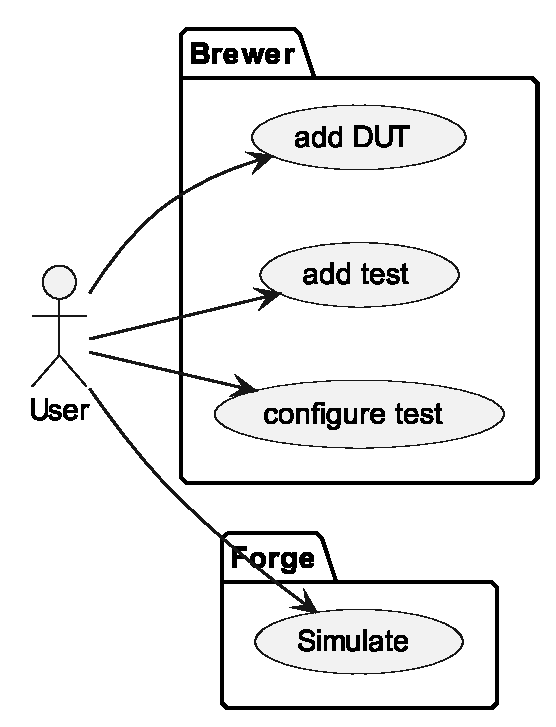
\includegraphics[width=.8\columnwidth]{out/plantuml/usecase2/usecase2.eps}
        \end{column}
    \end{columns}
\end{frame}
\begin{frame}{Separation of responsibility}
    \begin{columns}[T]
        \begin{column}{.45\textwidth}
            \textbf{The Brewer}
            \begin{itemize}
                \item Adding devices
                \item Handling test logic
                \item Preparing testbenches
            \end{itemize}
        \end{column}
        \begin{column}{.45\textwidth}
            \textbf{The Forge}
            \begin{itemize}
                \item Define command arguments
                \item Launch Verilator
                \item Collect Verilator output
                \item Handle concurrency
            \end{itemize}
        \end{column}
    \end{columns}
\end{frame}
\begin{frame}{The final workflow}
    \begin{center}
        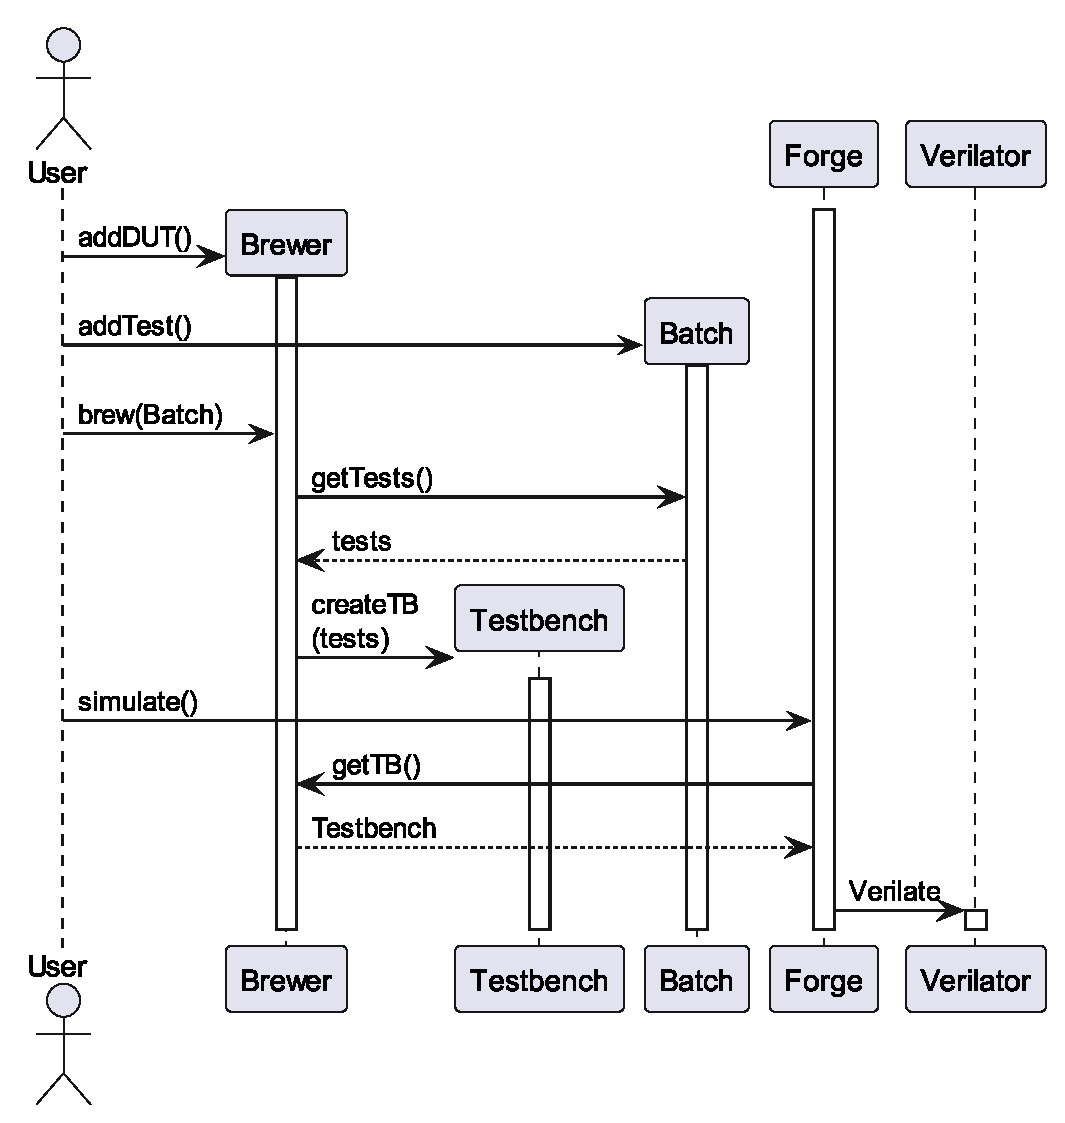
\includegraphics[height=.8\textheight]{out/plantuml/seq/sequenceDiag.eps}
    \end{center}
\end{frame}
\section{Implementation}
\subsection{Defining tests}
\begin{frame}{The program structure}
    \begin{center}
        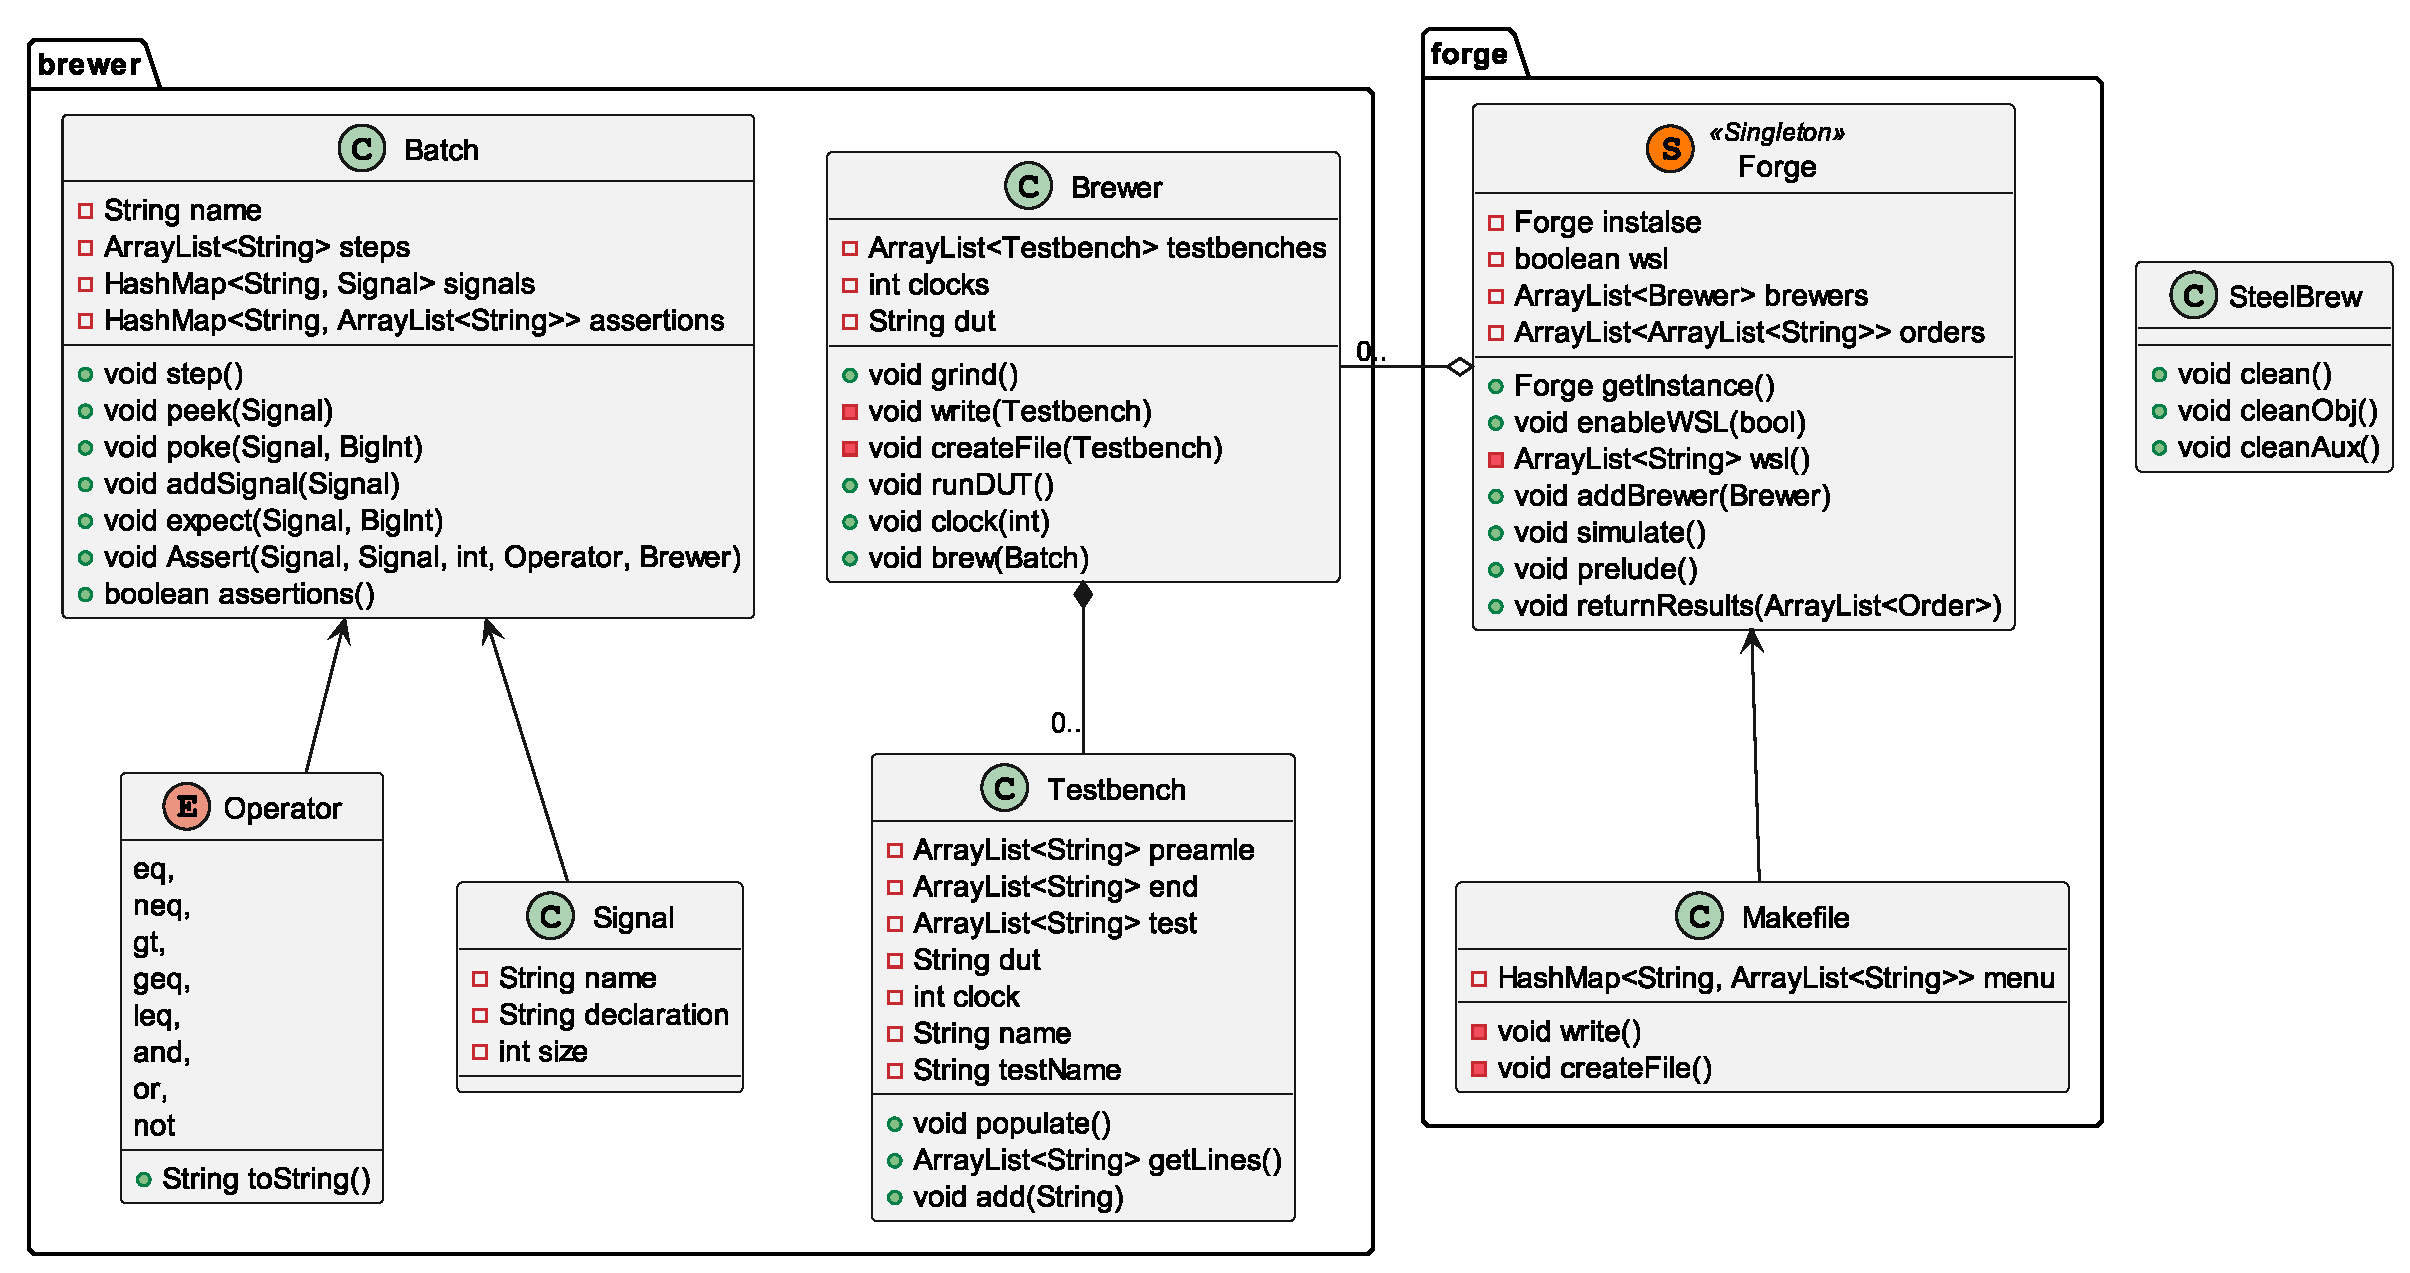
\includegraphics[height=.8\textheight]{out/plantuml/classDiag/classDiag.eps}
    \end{center}
\end{frame}
\begin{frame}[containsverbatim]{Batch}
    \begin{columns}[T]
        \begin{column}{.2\textwidth}
            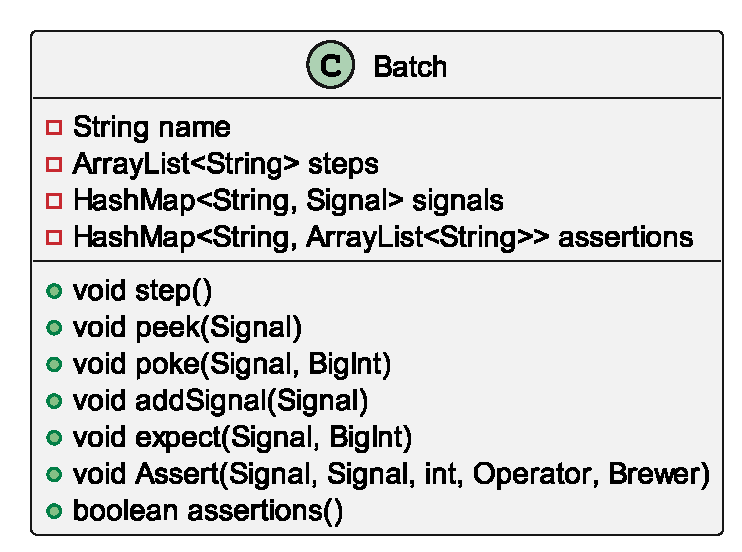
\includegraphics[width=\columnwidth]{out/plantuml/BatchClass/BatchClass.eps}
        \end{column}
        \begin{column}{.8\textwidth}
            \begin{minted}[fontsize=\footnotesize]{java}
    public void peek(Signal signal) {
        steps.add("std::cout << \"\\n Peek on " + signal.getName()
            + ": \" << (int)(dut->" + signal.getName()
            + ") << \" @ simtime: \" << sim_time << std::endl;\n");
    }
    public void poke(Signal signal, BigInteger integer) {
        steps.add("dut->" + signal.getName() + " = "
            + integer.intValue() + ";\n");
        steps.add("std::cout << \"\\n Poke on " + signal.getName()
            + ": " + integer.intValue()
            + "\"<< \" @ simtime: \" << sim_time << std::endl;\n");
    }
    public void expect(Signal signal, BigInteger integer) {
        steps.add("std::cout << \"\\n Expected " + integer.intValue()
            + " on " + signal.getName()
            + ". Recieved \"  << (int)(dut->" + signal.getName()
            + ") << \" @ simtime: \" << sim_time << std::endl;\n");
    }
            \end{minted}
        \end{column}
    \end{columns}
\end{frame}
\begin{frame}[containsverbatim]{Brewer}
    \begin{columns}[T]
        \begin{column}{.2\textwidth}
            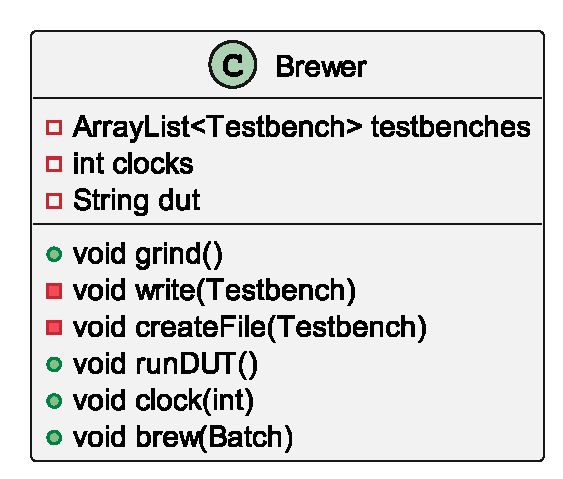
\includegraphics[width=\columnwidth]{out/plantuml/BrewerClass/BrewerClass.eps}
        \end{column}
        \begin{column}{.8\textwidth}
            \begin{minted}[fontsize=\footnotesize]{java}
public void brew(Batch batch) {
  Testbench testbench = new Testbench(dut, batch.getName(), clocks);
  if (batch.assertions()) {
    HashMap<String, ArrayList<String>> assertions = 
                                        batch.getAssertions();
    Set<String> functions = assertions.keySet();
    functions.forEach(f -> assertions.get(f).forEach(
                                        s -> testbench.addFunc(s)));
    testbench.add("    while (sim_time < MAX_SIM_TIME) {\n");
    ...
    functions.forEach(f -> testbench.add(f + "\n"));
    ...
  }
  ArrayList<String> steps = batch.getSteps();
  for (String step : steps) {
    testbench.add(step);
  }
  testbenches.add(testbench);
}
            \end{minted}
        \end{column}
    \end{columns}
\end{frame}
\begin{frame}[containsverbatim]{Testbench}
    \begin{columns}[T]
        \begin{column}{.2\textwidth}
            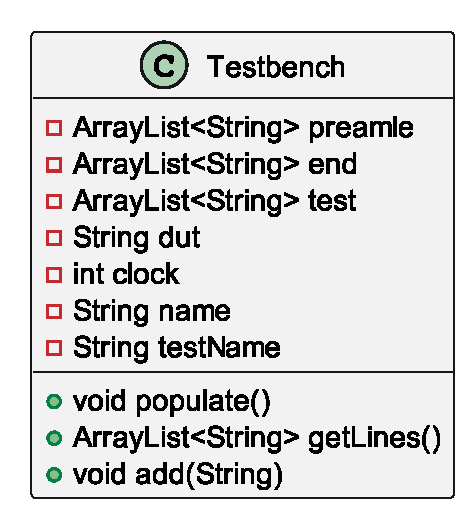
\includegraphics[width=\columnwidth]{out/plantuml/TestbenchClass/TestbenchClass.eps}
        \end{column}
        \begin{column}{.8\textwidth}
            \begin{minted}[fontsize=\footnotesize]{java}
public void populate() {
  preamble.add("#include <verilated.h>\n");
  preamble.add("#include \"V" + testName + ".h\"\n");
  ...
  main.add("int main(int argc, char** argv, char** env) {\n");
  main.add("    V" + testName + " *dut = new V" + testName + ";\n");
  main.add("    Verilated::traceEverOn(true);\n");
  ...
  main.add("    m_trace->open(\"waveform" + testName + ".vcd\");\n");
  ...
  end.add("    exit(EXIT_SUCCESS);\n");
}
public ArrayList<String> getLines() {
  ArrayList<String> returnList = new ArrayList<>();
  returnList.addAll(preamble);
  ...
  returnList.addAll(test);
  returnList.addAll(end);
  return returnList;
}
            \end{minted}
        \end{column}
    \end{columns}
\end{frame}
\subsection{Running tests}
\begin{frame}[containsverbatim]{Forge}
    \begin{columns}[T]
        \begin{column}{.2\textwidth}
            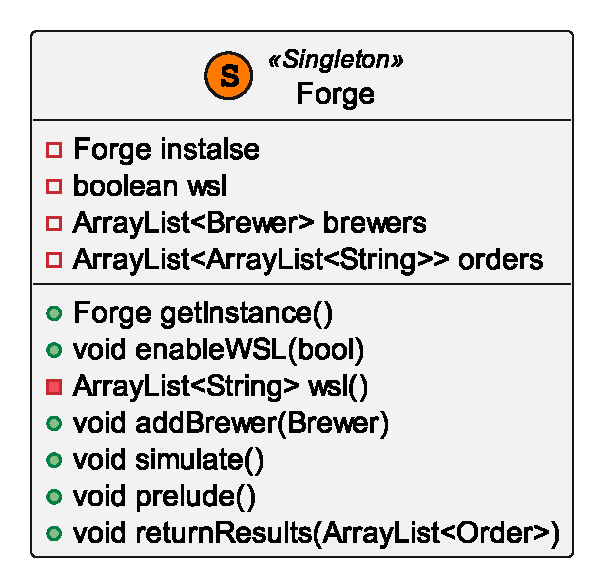
\includegraphics[width=\columnwidth]{out/plantuml/ForgeClass/ForgeClass.eps}
        \end{column}
        \begin{column}{.8\textwidth}
            \begin{minted}[fontsize=\footnotesize]{java}
public static void simulate() {
    prelude();
    ArrayList<String> tests = new ArrayList<>();
    brewers.forEach(b -> b.getTestbenches().forEach(
                    t -> tests.add(t.getName())));
    for (String test : tests) {
        ArrayList<String> list = new ArrayList<>();
        if (wsl) list = wsl();
        list.add("make");
        list.add(test);
        orders.add(list);
    }
    new Barista(orders);
}
public static void prelude() {
    brewers.forEach(b -> b.grind());
    new Makefile(brewers);
}
            \end{minted}
        \end{column}
    \end{columns}
\end{frame}
\section{Result}
\begin{frame}[containsverbatim]{Peeking and poking}
    \begin{columns}
        \begin{column}{.45\textwidth}
            \begin{minted}[fontsize=\footnotesize]{java}
Forge.enableWSL(true);
Brewer alu = new Brewer("alu");
Batch batch = new Batch("PeekPokeStep");
Signal signal = new Signal("in_valid", 1);
batch.addSignal(signal);
batch.peek(signal);
batch.poke(signal, BigInteger.ONE);
batch.step();
batch.peek(signal);
batch.step();
batch.poke(signal, BigInteger.ZERO);
batch.step();
batch.peek(signal);
batch.step();
batch.step();
alu.brew(batch);
Forge.simulate();
            \end{minted}
        \end{column}
        \begin{column}{.45\textwidth}
            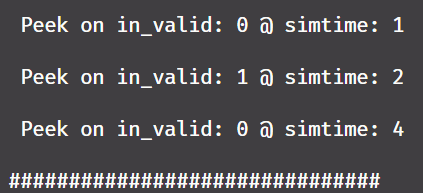
\includegraphics[width=\columnwidth]{graphics/peekpokestep.png}
        \end{column}
    \end{columns}
    \begin{center}
        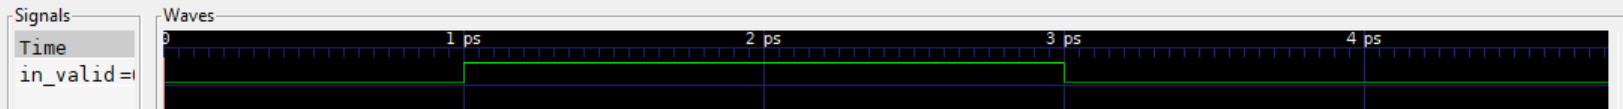
\includegraphics[width=.9\columnwidth]{graphics/peekpokestepWave.png}
    \end{center}
\end{frame}
\begin{frame}[containsverbatim]{Expect}
    \begin{columns}
        \begin{column}{.45\textwidth}
            \begin{minted}[fontsize=\footnotesize]{java}
Forge.enableWSL(true);
Brewer alu = new Brewer("alu");
Batch batch = new Batch("Expect");
Signal signal = new Signal("in_valid", 1);
batch.addSignal(signal);
batch.step();
batch.expect(signal, BigInteger.ONE);
batch.peek(signal);
batch.step();
alu.brew(batch);
Forge.simulate();
            \end{minted}
        \end{column}
        \begin{column}{.45\textwidth}
            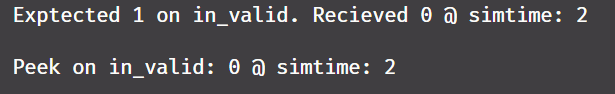
\includegraphics[width=\columnwidth]{graphics/expectConsole.png}
        \end{column}
    \end{columns}
\end{frame}
\begin{frame}[containsverbatim]{Concurrency}
    \begin{columns}
        \begin{column}{.45\textwidth}
            \begin{minted}[fontsize=\footnotesize]{java}
Forge.enableWSL(true);
Brewer alu = new Brewer("alu");
Brewer alu2 = new Brewer("alu2");
Batch batch = new Batch("PeekPokeStep");
Signal signal = new Signal("in_valid", 1);
batch.addSignal(signal);
batch.peek(signal);
batch.poke(signal, BigInteger.ONE);
batch.step();
batch.peek(signal);
batch.step();
batch.poke(signal, BigInteger.ZERO);
batch.step();
batch.peek(signal);
batch.step();
batch.step();
alu.brew(batch);
alu2.brew(batch);
Forge.simulate();
            \end{minted}
        \end{column}
        \begin{column}{.45\textwidth}
            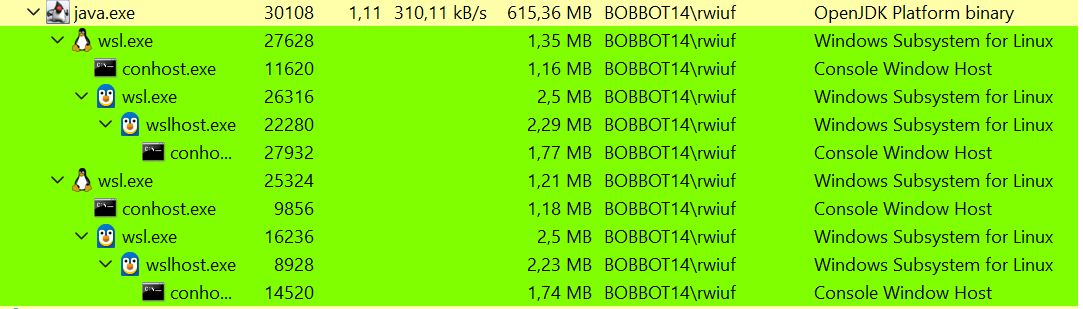
\includegraphics[width=\columnwidth]{graphics/concurrency.png}
        \end{column}
    \end{columns}
\end{frame}
\begin{frame}[containsverbatim]{Assertions}
    \begin{beamercolorbox}[sep=2em]{redbox}
        \textbf{No success (as such)}
    \end{beamercolorbox}
    But why?
    \begin{itemize}
        \item Assertions are mostly time independent
        \item Testbench works, but lacks sectioning
        \item Including a run loop for assertions exclude peek-poke-step
        \item The devil is in the details \mintinline{java}|functions.forEach(f -> testbench.add(f + "\n"));|
    \end{itemize}
\end{frame}
\section{Further development}
\begin{frame}{Further developments}
    \begin{itemize}
        \item Implement working assertions
              \begin{itemize}
                  \item Redo testbench for time independency \faCheckCircle
                  \item Fix assert \faCheckCircle
              \end{itemize}
        \item Employ Verilator multithreading \faTimesCircle
        \item Expand assertions with assume and cover logic \faTimesCircle
    \end{itemize}
\end{frame}
\section{Conclusion}
\begin{frame}{Conclusion}
    \begin{itemize}
        \item Did not reach final goal: Implementing Assertion Based Verification.
        \item SteelBrew communicates with Verilator
        \item SteelBrew uses Makefiles
        \item Basic testing methods
        \item Handles concurrent execution
        \item Handles multiple DUT's and test routines for each
    \end{itemize}
\end{frame}
\section*{}
\begin{frame}[plain,standout]{Q\&A}
    \begin{columns}[c]
        \begin{column}{.3\textwidth}
            \begin{center}
                Questions?
            \end{center}
        \end{column}
        \begin{column}{.5\textwidth}
            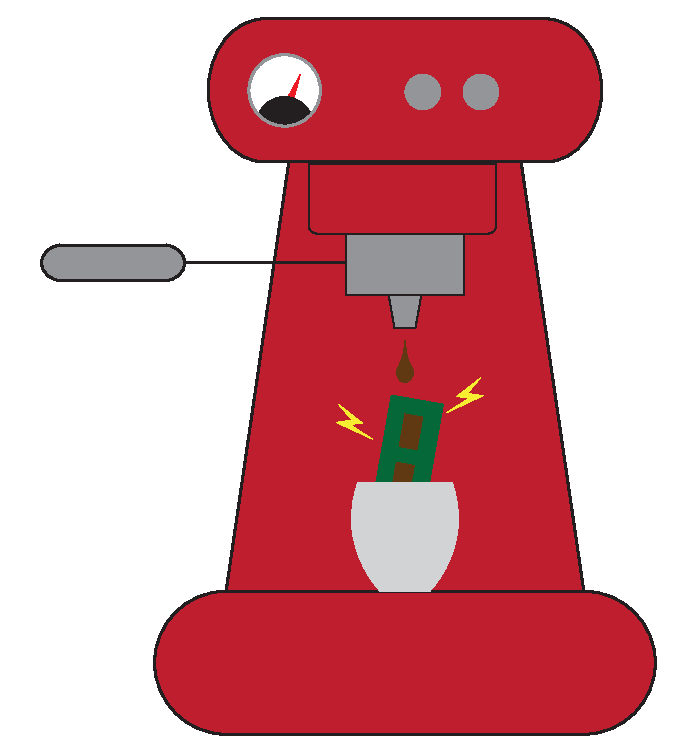
\includegraphics[width=.8\columnwidth]{graphics/steelbrew.eps}
        \end{column}
    \end{columns}
\end{frame}
\begin{frame}[plain,standout]{Assertion fix}
    \begin{columns}[c]
        \begin{column}{.3\textwidth}
            \begin{enumerate}
                \item Do a while in each testbench
                \item Assertion methods defined before main method
                \item Each test inclosed in simulation-time condition
                \item Assertion method runs every cycle
            \end{enumerate}
        \end{column}
        \begin{column}{.5\textwidth}
            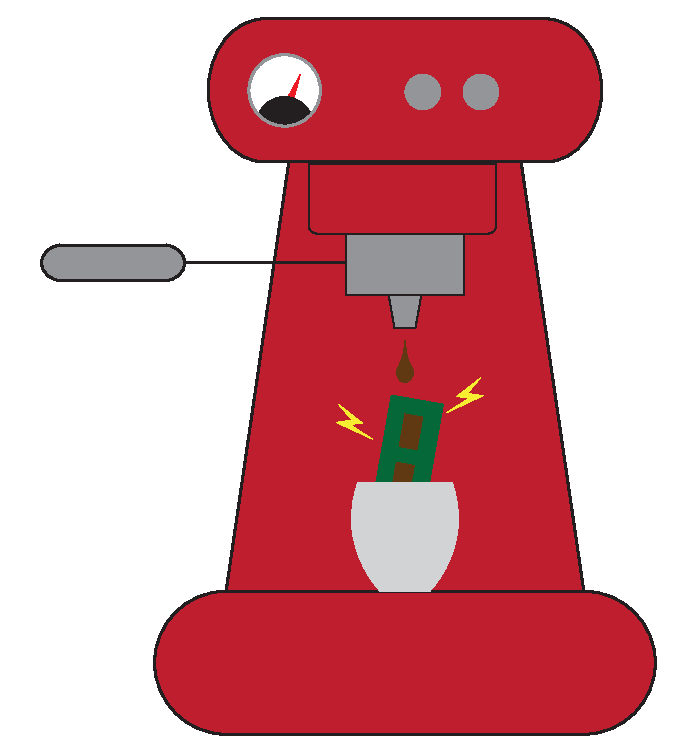
\includegraphics[width=.8\columnwidth]{graphics/steelbrew.eps}
        \end{column}
    \end{columns}
\end{frame}
\end{document}